\documentclass[11pt,singlecolumn]{scrartcl}
\usepackage[masterthesis]{systems-cover}
\usepackage{amsmath,amssymb,amstext}
\usepackage[utf8]{inputenc}
\usepackage[english]{babel}
\usepackage{fancyhdr}
\usepackage{graphicx}
\usepackage[capposition=bottom]{floatrow}
\usepackage{listings}
\usepackage{url}
\usepackage{titlesec}

\titleformat*{\section}{\LARGE\bfseries}
\titleformat*{\subsection}{\Large\bfseries}
\titleformat*{\subsubsection}{\large\bfseries}

\lstset{frame=tb,
  language=Java,
  aboveskip=3mm,
  belowskip=3mm,
  showstringspaces=false,
  columns=flexible,
  basicstyle={\small\ttfamily},
  numbers=left,
  numberstyle=\tiny,
  breaklines=true,
  breakatwhitespace=true,
  tabsize=3
}

\pagestyle{fancy}
\fancyhf{}
\fancyhead[LE,RO]{A High-level Graph Query Language Interface for Differential Dataflow}


\fancyfoot[RE,lO]{Master Thesis}
\fancyfoot[LE,RO]{\thepage}

\renewcommand{\headrulewidth}{2pt}
\renewcommand{\footrulewidth}{1pt}

\covernum{164}
\covertitle{A High-level Graph Query Language Interface for Differential Dataflow}
\coverauthor{Lukas Striebel}
\coverdate{October 2016 - April 2017}
\coversupervisedby{Prof.\ Timothy Roscoe\\Dr. Ioannis Liagouris\\Dr. Desislava Demitrova\\Moritz Hoffmann}


\begin{document}

\hspace{60mm}
\begin{center}
 \textbf{Abstract} \end{center}
In today's business world, Social Networks have become one of the most important if not the most important platforms to advertise and attract new customers. Thus, graph databases have been increasing in popularity in comparison to traditional relational databases. This tendency has given birth to the need of powerful and graph datawarehouses and query evaluators. In this thesis, we present Qlidaf, an Interface of the Property Graph Query Language for Diffrerential Dataflow.


\clearpage
\tableofcontents
\clearpage
\listoffigures
\clearpage
\section{Introduction}
\subsection{Motivation}
In our modern digital age, the Internet is the largest centre of data and knownledge. The websites of large companies are accessed thousands of times a day. In order to cope with this huge amount of client requests, large sever farms were built. In these farms, hundreds of servers and switches are connected and request have to travel across multiple machines until they are answered. Thus, the need for a system that directs and balances the huge amount of request arises. The first step to deal with this challenge is to model this complicated network of computers as a property graph. In a second step, an algorithm determines how the request should best be directed in order to not overload any part of the network. This thesis focuses on the second step and proposes a program that can evaluate queries on a property graph, in order to determine weak links and find the optimal distribution of the work load.
\subsection{Structure of the Thesis}
The Thesis has the following structure:\\
First, we give an overview of the technologies used in the Thesis in Section 2.\\
We continue by giving a detailed explanation of the query parser  in Chapter 3. In Section 4, we explain how the program sets up the dataflows according to the query. Next, we describe the experiments that were run in order to determine the performance of the program in Chapter 5. Finally, we draw our conclusion, provide an outlook and show potential for future work.
\clearpage

\section{Background}
In this section, all the relevant technologies used in the Thesis are explained.
\subsection{The Property Graph Query Language}

The Property Graph Query Language (PGQL) was developed by Oskar van Rest at Oracle. \cite{vanRest:2016} PGQL enables developers to write intuitive path queries over a property graph. A PGQL query consists of 4 clauses, two of them are optional.
\begin{itemize} 
\item Path Clause (optional)
\item Select Clause (required)
\item Where Clause (required)
\item Solution Modifier Clause (optional)
\end{itemize}

In the Path Clause custom path patterns are defined, which are to be used again in the Where Clause.\\
\textbf{Example:}\\
\begin{lstlisting}
PATH connects_to := (:Generator) -[:has_connector]-> (:Connector WITH status = 'OPERATIVE') <-[:has_connector]- (:Generator)
 \end{lstlisting}
The Select Clause bears great similarity to the SQL one. Here, the set of properties one wishes to retrieve is defined. Possible Selections are either\\
\begin{itemize} 
\item everything, indicated by the use of * 
\item certain attributes of edges and/or vertices
\item Aggregation of certain attributes of edges and/or vertices.
\end{itemize}
 Currently, there are five types of aggregations supported:\\
 \begin{itemize} 
\item COUNT, returns the number of tuples in the solution 
\item MAX, returns the maximum value of an attribute in any tuple. The specified attribute has to be numeric.
\item MIN, returns the minimum value of an attribute in any tuple. The specified attribute has to be numeric.
\item SUM, returns the sum of an attribute over all the tuples. The specified attribute has to be numeric.
\item AVG, returns the average of an attribute over all the tuple. The specified attribute has to be numeric.
\end{itemize}
\textbf{Example:}\\
\begin{lstlisting}
SELECT v.name, AVG(v.age)
 \end{lstlisting} 
The most complex part of the query is the Where Clause. In this section, all the requirements that the edges and vertices of the result set have to fulfill are specified.
\textbf{Example:}\\
\begin{verbatim}
  WHERE v.name = 'Alice', v.age > 30
\end{verbatim}

The official PGQL Specifications can be accessed online at \cite{PGQLSpec}
\clearpage
\subsection{Dataflow Programming}
Dataflow oriented programming is a programming paradigm that models a program as a directed graph of data flowing between operations.

\clearpage

\subsection{Differential Dataflow}

Developed by Frank McSherry at Microsoft, Differential dataflow is a data-parallel programming framework designed to efficiently process large volumes of data and to quickly respond to arbitrary changes in input collections.\cite{Differential}\\
Differential Dataflow is an extension of Timely Dataflow, which was also created by Frank McSherry. \cite{GitTimely}
Rather than rewriting the entire data every time a change occurs, Differential Dataflow only keeps track of the changes made to the data. This allows for huge timesavings when executing the same operation multiple times on different data, since the results of previous computations can be reused.\\\\
Differential Dataflow is open-source and available for download at \cite{GitDiff}.
\clearpage

\subsection{The Rust Programming Language}
Rust is a fairly new programming language. It's origin lies with the Mozilla Company, where former employee Graydon Hoare started development in 2006. In the year 2009, Mozilla offically began sponsering the project.\\
Rust has been praised as it combines guaranteed memory safety with minimal runtime. Other prominent features are zero-cost abstractions, move semantics, threads without data races, trait-based generics, pattern matching, type inference and efficient C bindings\cite{RustLang}. The Rust compiler is self-hosted, meaning it is written in Rust as well. Rust won the Award for Most Loved Programming Language in 2016, host by the Stack Overflow Community.
Rust is completly opensource, and a big part of the code was written by members of the community.
\clearpage

\subsection{Nom}
The Parser is build using nom, \cite {Nom}. Nom was developed by Geoffroy Couprie. It is a byte oriented, zero copy, streaming Parser Library written in Rust. The library provides macros, functions and enums which faciliate the parsing process.\\\\
The most commonly used macros were:
\begin{itemize} 
\item do\_parse!: Takes a list of parsers as inputs and applies them sequentially, finally returns a tupel.
\item alt\_complete!: Takes a set of parsers as input and applies them until one succeeds. Returns the result of the first successful parser.
\item opt!: Takes a parsers as input and makes it optional. Returns None if parser was unsuccessful or Some otherwise.
\item tag!: Parses a specific String. Aborts if the String is not found.
\item named!: Faciliates the creation of new custom parsers.
\item many0!: Applies the parser 0 or more times.
\item many1!: Applies the parser 1 or more times. 
\end{itemize}

Nom is open-source and available for download at \cite{GitNom}.

\clearpage

\section{Parser}
In the following, we describe how our parser is build. As mentioned in Section 2.1, the Parser has to recognize the following 4 clauses: Path definitions, select, where, solution modifier.
\\The main parse function therefore looks:
\begin{lstlisting}
named!(pgql_query<Query>,
	do_parse!(
		paths: opt!(paths) >>
		space >>
		select: select_clause >>
		space >>
		vvhere: where_clause >>
		space >>
		solmod: opt!(solutionModifier) >>
		(Query { select: select, vvhere: vvhere, paths: paths, solmod: solmod})
     )
);
 \end{lstlisting} 
\clearpage

\subsection{Path Clause}

The Path Clause is a list of definitions. Each Path definition starts with a name, followed by `:=' and then a path description. The path defined in this clause can then be reused in the Where Clause. One of many difficulties encountered while writing the parser, is the ability to differentiate between a single path definition and multiple ones, seperated by commas.


\clearpage
\subsection{Select Clause}
The Select Clause of PGQL is very similar to the SQL one. Started by the keyword `Select', a list of attributes is provided. Attributes may be renamed with the keyword `as'. Aggregate functions like `Sum', `Avg' etc. may also be accessed.

\clearpage

\subsection{Where Clause}
The Where Clause consists of a list of Constraints. Each constraint defines either a path or value requirement that has to be fulfilled by the respective vertex or edge.
 
 \subsubsection{Path Constraints}
 Path Constraints are patterns, which are matched against the graph. If a set vertices does not fit the pattern, it is discarded.\\
 A typical Path Constraint requires a vertex to have certain edges to other vertices. For example, the constraint: (v) -> (u) requires that the vertex v has a direct edge to the vertex u.\\\\Vertices are absoultly essential for the path constraints. A Vertex is delimited by brackets () and its properties are specified inside the brackets (or at a later point in time). There are three parameteres, all of them are completly optional:\\
 \begin{itemize}
 \item The name of the vertex. If no name is provided, the vertex is anonymous.
 \item A set label constraints, recognized by the : sign. Label constraints differ from value constraints
 \item A set of inlined value constraints, recognized by the keyword WITH. This is basically just syntatic sugar, for example, the two formulation (v WITH age \textgreater 10) and (v), v.age \textgreater 10 are completly equal.
 \end{itemize}
 
\textbf{Code sample}
\begin{lstlisting}
named!(query_vertex<Vertex>,
    delimited!(
        char!('('),
        do_parse!(
            vertex_name: opt!(char_only) >> 
            opt!(space) >>
            label: opt!(label_constraint) >>
            opt!(space) >>
            inlined: opt!(inlined_constraints) >>
            ({
                
                let mut constraints: Vec<Expr> = match inlined {
                    Some(value) => value,
                    None => Vec::new()
                };

                match label {
                    Some(value) => {constraints.push(value);},
                    None => {}
                }

                match vertex_name {
                    Some(name) => {Vertex{name: String::from(name), anonymous: false, constraints: constraints }},
                    None => Vertex{name: String::from(""), anonymous: true, constraints: constraints }
                }
            })                
        ),
        char!(')')
  )
);
 \end{lstlisting} 
 
 The connection between two vertices can be a very simple or a very sophisticated edge with many attributes. An edge is defined by an arrow sign -\textgreater and its properties are specified inside the brackets (or at a later point in time). There are three parameteres, all of them are completly optional:\\
 \begin{itemize}
 \item The name of the vertex. If no name is provided, the vertex is anonymous.
 \item A set label constraints, recognized by the : sign. Label constraints differ from value constraints
 \item A set of inlined value constraints, recognized by the keyword WITH. This is basically just syntatic sugar, for example, the two formulation (v WITH age \textgreater 10) and (v), v.age \textgreater 10 are completly equal.
 \end{itemize}
 
\textbf{Code sample}
 \begin{lstlisting}
named!(query_edge<Edge>,
        alt_complete!(
            tag!("-->") => { |_| Edge {name: String::from(""), inverted: false, constraints: Vec::new() } } |
            tag!("->") => { |_| Edge {name: String::from(""), inverted: false, constraints: Vec::new() } } | 
            delimited!(
                tag!("-["),
                do_parse!(
                    edge_name: opt!(char_only) >> 
                    opt!(space) >>
                    label: opt!(label_constraint) >>
                    opt!(space) >>
                    inlined: opt!(inlined_constraints) >>
                    ({
                        
                        let mut constraints: Vec<Expr> = match inlined {
                            Some(value) => value,
                            None => Vec::new()
                        };

                        match label {
                            Some(value) => {constraints.push(value);},
                            None => {}
                        }

                        match edge_name {
                            Some(name) => {Edge{name: String::from(name), inverted: false, constraints: constraints }},
                            None => Edge{name: String::from(""), inverted: false, constraints: constraints }
                        }
                    })                
                ),
                tag!("]->")
 );
 \end{lstlisting}
 \clearpage
 \subsubsection{Value Constraints}
 Value Constraints are constraints on attributes of the Vertex, e.g. name = `Alice' or age \textless  40. Every Value Constraint has to include one or multiple vertex attributes, and one or more Literals. Literals are raw values, and come in 3 types:
 \begin{itemize} 
\item Strings e.g. `Alice'
\item Floats e.g. 40
\item Booleans, which are either true or false
\end{itemize}
 
 \begin{lstlisting}
pub enum Literal {
    Str(String),
    Float(f32),
    Boolean(bool),
} 
 
named!(literal<Literal>,
    alt_complete!(
        float       => { |f| Literal::Float(f)             } |
        boolean     => { |b| Literal::Boolean(b)           } |
        string      => { |s| Literal::Str(String::from(s)) } 
            
    )
);
 \end{lstlisting}
 
 
 \clearpage
 
 \subsection{Solution Modifier Clause}
 
 The Solution Modifier Clause consists of three parts: 
  \begin{itemize} 
\item GroupBy Clause
\item OrderClause
\item Offset and Limit Clause
\end{itemize}
 All clauses are optional and can be omitted. 
 
\clearpage



\section{Query Evaluation}
In this chapter we will discuss how we construct the dataflow from our queries.
\subsection{Graph Loader}
The Loading of the graph plays a major part of the entire program execution time. To load a graph from a text file into differential Dataflow, an entirely new parser had to be written. This parser was also built using nom. In order fo it to properly recognize a graph, the graph has to be supplied in the Vertex-Edge-List format\cite{EdgeList}. This format gives us a text file (.txt), which contains two lists. First, all the vertices and their attributes are described. The vertices are ordered ascing according to their ID. The IDs have to start at 1 and must be continuous.\\\\
\textbf{Small sample graph}
\begin{lstlisting}
1 * { 'Server' }             name:'center'   ip:'192.168.0.0'   ram:4
2 * { 'VM' }                 name:'node1'    ip:'192.168.0.1'	ram:8
3 * { 'Firewall' 'VM' }      name:'node2'    ip:'192.168.0.2'	ram:16.5
4 * { 'Host' 'Server' 'VM' } name:'node3'    ip:'192.168.0.3'	ram:32.5
5 * { 'Switch' }             name:'node4'    ip:'192.168.0.4'	ram:64.5
1 2 'connectss' bandwidth:1.5 utilization:0.14
2 3 'connects' bandwidth:2.1 utilization:0.22
2 4 'connects' bandwidth:1.1 utilization:0.38
4 5 'connects' bandwidth:1.3 utilization:0.58
\end{lstlisting}
\clearpage
\subsection{Construction of the Dataflow}
The biggest challenge in the thesis was translating the PGQL query into a dataflow. As described in chapter 3, a query contains a vector of projections and a vector of constraints. We chose to apply the projections at the vey latest point in time. Thus, our evaluation begins with the second vector.\\\\
\subsection{Constraint sorting}
First, we iterate through the vector and sort the constraints by type:\\
\begin{itemize}
\item If the constraint is a path pattern, it is put into a seperate vector.
\item If the constraint is an expression, we determine the name of the involved vertex or edge by recursively exploring the expression. Once the variable name is known, the expression is then pushed into a Hashmap of Vectors. For each variable there exists a seperate vector with expressions. This grouping helps tremendously when filtering the vertex set later on.
\end{itemize}
\textbf{Code sample}
\begin{lstlisting}
for constraint in &vvhere{
                match constraint {
                    &Constraint::PathPattern(ref pattern) => connections.push(pattern),
                    &Constraint::Expr(ref expr) => {
                        let name = explore_expr((*expr).clone());
                        let mut new = false;
                        match selections.get_mut(&name) {
                            Some(vec) => vec.push((*expr).clone()),
                            None => new = true,
                        }
                        if new {
                            selections.insert(name, vec![(*expr).clone()]);
                        }
                    },
                }
            }
\end{lstlisting}
\subsection{Constructing an execution plan}
Once we have iterated over the entire vector, we begin the construction of an execution plan. We iterate through all the path patterns (we have stored them previously in a seperated vector) and make a decision how to construct the plan. There are three possibilities:
\begin{itemize}
\item Both the source and the target of the edge have not appeared before. In this case, we pull the source and the target set and join them with the edge set. 
\item The source of the edge has already appeared before. In this case, we pull the target set, map the result we carried onto the correct id and then join them with the edge set.
\item Both the source and the target of the edge have appeared before. In this case, we are dealing with a loop in the query. Thus, we do not need to join any sets, but we can just enforce an additional constraint on the ids.
\end{itemize}
\textbf{Code sample}
\begin{lstlisting}
for connection in connections {
                if !used_fields.contains(&connection.source.name) {
                    used_fields.insert(&connection.source.name);
                    used_fields.insert(&connection.target.name);
                    names.insert(&connection.source.name, ids);
                    ids = ids + 1;
                    names.insert(&connection.target.name, ids);
                    ids = ids + 1;

                    let mut new = false;
                    match selections.get_mut(&connection.source.name) {
                            Some(mut vec) => vec.append(& mut connection.source.constraints.clone()),
                            None => new = true,
                    }
                    if new {
                            selections.insert(connection.source.name.clone(), connection.source.constraints.clone());
                    }
                    new = false;
                    match selections.get_mut(&connection.target.name) {
                            Some(mut vec) => vec.append(& mut connection.target.constraints.clone()),
                            None => new = true,
                    }
                    if new {
                            selections.insert(connection.target.name.clone(), connection.target.constraints.clone());
                    }

                    execution_plan.push(
                        PhyPlan{ 
                            name: vec![connection.source.name.clone(), connection.target.name.clone()],
                            left: connection.source.name.clone(),
                            right: connection.target.name.clone(),
                            join_id: 0,
                            join: true,
                            filter_id: 100,
                            constraints: connection.edge.constraints.clone(),
                        }
                    );
                }
                else if !used_fields.contains(&connection.target.name) {
                    used_fields.insert(&connection.target.name);
                    names.insert(&connection.target.name, ids);
                    ids = ids + 1;

                    let mut new = false;
                    match selections.get_mut(&connection.target.name) {
                            Some(mut vec) => vec.append(& mut connection.target.constraints.clone()),
                            None => new = true,
                    }
                    if new {
                            selections.insert(connection.target.name.clone(), connection.target.constraints.clone());
                    }
                    execution_plan.push(
                        PhyPlan{ 
                            name: vec![connection.source.name.clone(), connection.target.name.clone()],
                            left: connection.source.name.clone(),
                            right: connection.target.name.clone(),
                            join_id: *names.get(&connection.source.name).unwrap(),
                            join: true,
                            filter_id: 100,
                            constraints: connection.edge.constraints.clone(),
                        }
                    );
                }
                else {
                    execution_plan.push(
                        PhyPlan{ 
                            name: vec![connection.source.name.clone(), connection.target.name.clone()],
                            left: connection.source.name.clone(),
                            right: connection.target.name.clone(),
                            join_id: *names.get(&connection.source.name).unwrap(),
                            join: false,
                            filter_id: *names.get(&connection.target.name).unwrap(),
                            constraints: connection.edge.constraints.clone(),
                        }
                    );
                }

            }
\end{lstlisting}
\subsection{Selection on the vertex set}
The next step is to apply all the selections we have sorted beforehand on the vertex set. For each non-anonymous vertex, we filter the entire set and save the result in a Hashmap. The key in this Hashmap is the name of the vertex.
\textbf{Code sample}
\begin{lstlisting}
for (name, filter) in selections {
                let result = vertices.filter(move |x| {
                    check_node(&x, &filter)
                });

                plans.insert(name, result);
            }
\end{lstlisting}
\subsection{Executing the plan}
\textbf{Code sample}
\begin{lstlisting}
let mut result = None;
                for step in execution_plan {

                    //let constraints = &step.constraints 
                    
                    if step.join && step.join_id == 0 {
                        let sources = match plans.get(&step.left){
                            None => vertices,
                            Some(list) => list,
                        };

                        let targets = match plans.get(&step.right){
                            Some(list) => list,
                            None => vertices,
                        };
                        result =    Some(sources.map(|x| (x.id, x))
                                    .join(&edges.filter(move |x| check_edge(&x, &step.constraints))
                                    .map(|x| (x.source,x.target)))
                                    .map(|(_,v1,v2)| (v2,v1))
                                    .join(&targets.map(|x| (x.id, x)))
                                    .map(|(_,v1,v2)| vec![v1,v2]));
                    }
                    else if !step.join {
                        let int = step.join_id;
                        let int2 = step.filter_id;
                        result = Some(result.unwrap().map(move |x| (x[int].id, x))
                                .join(&edges.filter(move |x| check_edge(&x, &step.constraints))
                                .map(|x| (x.source,x.target)))
                                .filter(move |x| {let &(ref key, ref vec, ref id) = x; vec[int2].id == *id})
                                .map(|(_,v1,_)| v1));

                    }
                    else {                 
                        let targets = match plans.get(&step.right){
                            Some(list) => list,
                            None => vertices,
                        };
                        result = Some(result.unwrap().map(move |vec| (vec[step.join_id].id, vec))
                                .join(&edges.filter(move |x| true)//check_edge(&x, &step.constraints))
                                .map(|x| (x.source,x.target)))
                                .map(|(_,v1,v2)| (v2,v1))
                                .join(&targets.map(|x| (x.id, x)))
                                .map(|(_, mut v1,v2)| {v1.push(v2);v1}));   
                    }
                }
 \end{lstlisting} 
\subsection{Applying the projection and aggregation}
\textbf{Code sample}
\begin{lstlisting}
for projection in &select{
                            match projection {
                                &SelectElem::Star => {
                                    list.inspect(|&(ref x,_)| println!("{:?}", x));
                                },
                                &SelectElem::Attribute(ref attr) => {
                                    //let strng = string_to_static_str(attr.name.clone());
                                    let field = string_to_static_str(attr.field.clone());
                                    let id = *(names.get(&attr.name).unwrap());
                                    list.inspect(move |&(ref x,_)| println!("{:?}", x[id].get(&field.into()).unwrap()));
                                    
                                    
                                },
                                &SelectElem::Aggregation(ref aggr) => {
                                    match aggr {
                                        &Aggregation::Count(ref attr) => {
                                                list.map(move |x| (1, x)).group(move |key, vals, output| {
                                                        let mut count = 0;
                                                        for _ in vals {
                                                            count = count + 1;
                                                        }                                                        
                                                        output.push(((),count));
                                                    }).inspect(|&(_, ref x)| println!("{:?}", x));
                                                
                                            }
 \end{lstlisting} 
\clearpage


\section{Results and Discussion}

\subsection{Hardware}
All the experiments were conducted on an ETH server (exact model?). This machine possesses 4 x 12 AMD Opteron 6174 processors, each one running at 2.2 GHz. The operating System was Debian 7.0 and the installed memory was 128 GB of RAM.
\subsection{Topologies}
We select two distinctly different
topologies: fattree~\cite{FatTree} and jellyfish~\cite{Jellyfish}. fattree is a modification of the leaf-spine structure, commonly found in datacenters, and it is thus a practically deployable solution. jellyfish is inspired by work on random graphs showcasing that random structures can deliver shorter average paths but is more of an ideal-case reference rather than a realistic topology.
In the experiment, four different topologies were used:\\\\
\textbf{Large Fattree} \quad  The large fattree topology is the largest one of the four topologies. It contains 55'000 vertices, of which 2'880 are switches. Furthermore the graph posses a total of 50'000 bidirectional edges. Since one bidirectional edge is represented by two directed edges, there are a total of 100'000 edges in the collection.\\\\
\textbf{Small Fattree} \quad The small fattree topology has the same vertices to edge ratio as the large fattree, but it is overall much smaller. It contains 17'665 vertices, of which 1'280 are switches. Furthermore the graph possesses a total of 16' 400 bidirectional edges. (needs better formulation) \\\\
\textbf{Large Jellyfish} \quad  The large jellyfish topology matches the large fattree in terms of vertices, but contains far less edges. It contains 56'160 vertices, of which 864 are switches. Furthermore the graph possesses a total of 6'910 bidirectional edges. (needs better formulation)\\\\
\textbf{Small Jellyfish} \quad The small jellyfish topology is the smallest one of the four topologies. It contains 16'770 vertices, of which 390 are switches. Furthermore the graph possesses a total of 2'145 bidirectional edges. (needs better formulation)
\subsection{Expectations}
In all topologies, weight is an attribute of the edges and uniformly distributed from 1 to 9. Consequently, the selection 'weight \textless 2' will therefore remove around 89\% of all edges. A lesser amount of edges immensely shortens the duration of any subsequent join process.\\ Since joining the entire vertex and edge set is a very costly operation, it is possible that queries with multiple, but restricted joins are faster than such, which contain fewer joins, but do not include any restrictions on the edge set. \\\\
Furthermore, it is important to consider the fact that the attributes of vertices and edges in a Differential Dataflow Collection are stored in a Vector of (String, Literal) tuples. We chose this suboptimal implementation since Differential Dataflow does not aprreciate HashMaps at all. However, in order to do a selection on either set, this Vector has to be transformed back into a HashMap for each edge respectively vertex. This process can be quite timeconsuming, therefore the more selections a query contains, the slower it expected to be.\\\\
It should also be noted that one single edge in the query triggers two joins in the evaluation. Reason being that we have to join the edge collection twice with the vertex collection, in order to determine all adjacent vertices of a given vertex.\\\\\\
In total, we ran seven different queries, with each subsequent query being more complex than the preceding one. For each query the resulting dataflow is drawn on the following pages. The numbers on the edges indicate the size of (intermediate) result set on the large fattree.\clearpage
\subsection{Overview}
\begin{figure}[H]
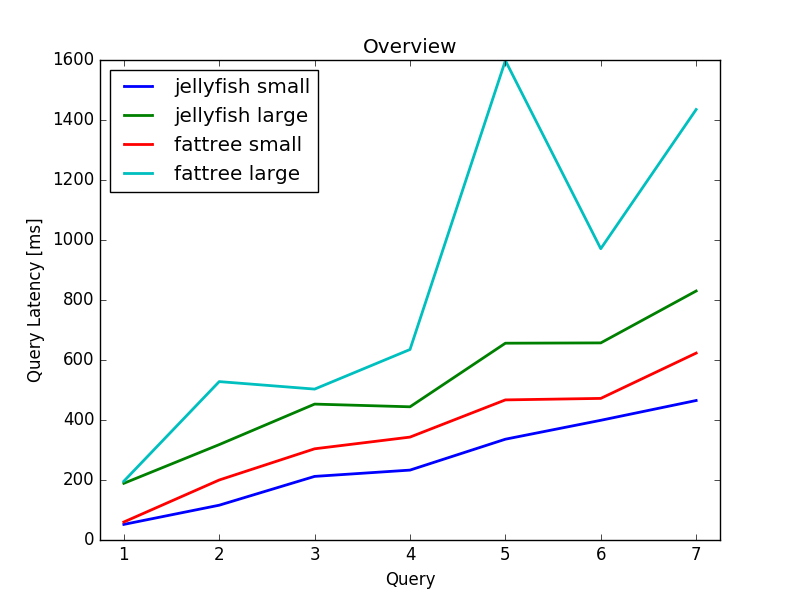
\includegraphics[width=1\textwidth]{ov}
\caption{An overview of the seven queries, run with 32 workers}
\end{figure}
Throughout all seven queries, the following pattern is noticeable:\\
The influence of the number of workers behaves unexpectedly, especially for queries 1,4 and 6. In a perfect world, the query latency would be inversely proportional to the number of workers. However, we only observe this behaviour for query 5, and only for the fattree topologies.\\More often than not, an increase of worker threads leads to a higher latency, especially when the latency is already quite low, around the 50 to 200 millisecond range. We reason that this happens because at that level, the communication overhead dominates the time savings achieved by parallelism. This claim is additionally supported by the fact, that query 5 has one of the longest latencies, ranging up to 10 seconds. When evaluating queries with lower latency, the contention between the workers increases and we frequently observe that the best performance is achieved when running the query with just a single worker.\\
The following pages contain the dataflows executing the query and the evaluation times distribution for each of the seven queries

\clearpage

\subsection{Query 1}
\begin{verbatim}
SELECT u.name WHERE u.label() = 'switch', u.position = 'access'
\end{verbatim}

\textbf{Peak Memory: 377'840 kb}\\
\textbf{Result size: 1'152} \\
2 simple selections, 0 joins. One pass through the vertices collection is enough to produce the result.\\\\
\textbf{Dataflow}
\begin{figure}[H]
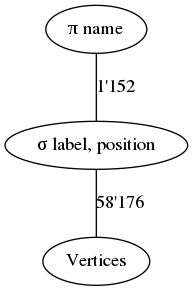
\includegraphics[width=0.4\textwidth]{graph1}
\caption{Dataflow Query1}
\end{figure}
\clearpage
\begin{figure}[!tbp]
  \centering
  \RawFloats
  \begin{minipage}[b]{0.5\textwidth}
    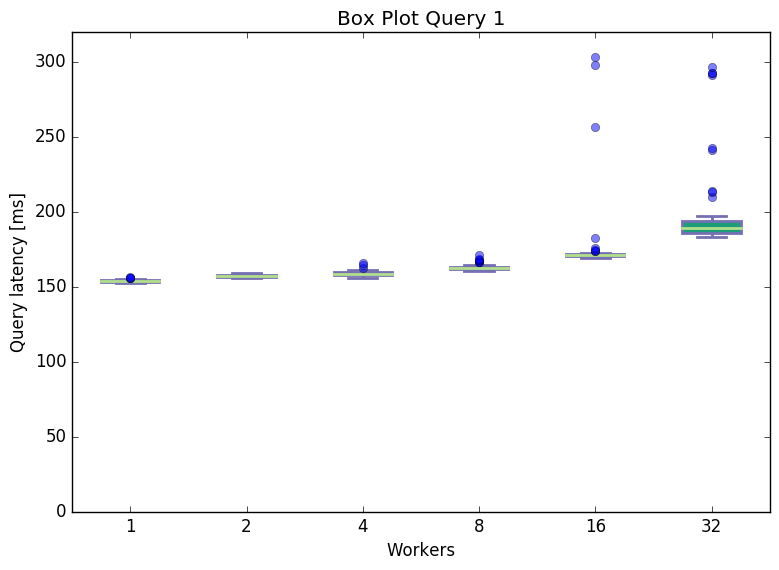
\includegraphics[width=\textwidth]{boxesfl/q1}
    \captionof{figure}{Large Fattree}
  \end{minipage}
  \hfill
  \begin{minipage}[b]{0.5\textwidth}
    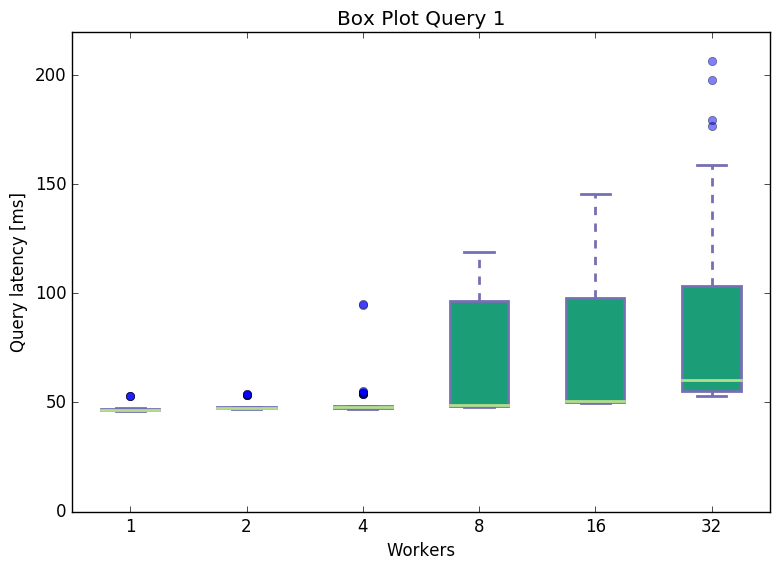
\includegraphics[width=\textwidth]{boxesfs/q1}
    \captionof{figure}{Small Fattree}
  \end{minipage}
\end{figure}
\begin{figure}[!tbp]
  \centering
  \RawFloats
  \begin{minipage}[b]{0.5\textwidth}
    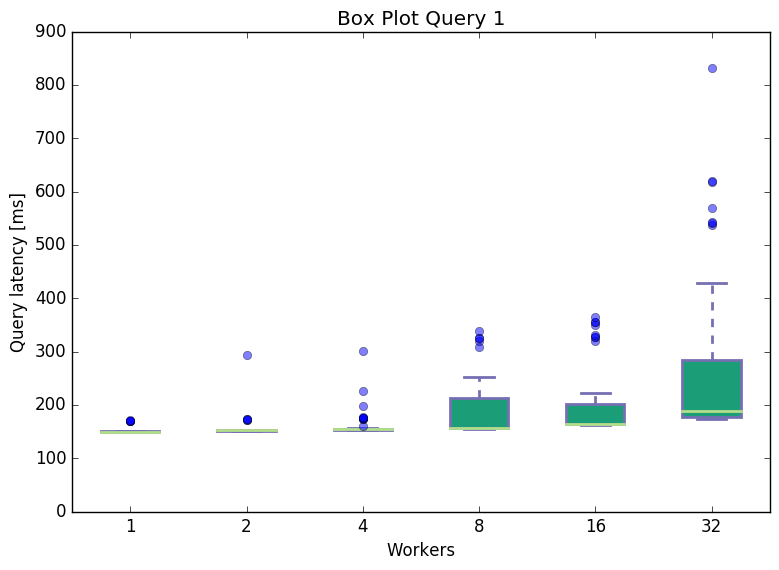
\includegraphics[width=\textwidth]{boxesjl/q1}
    \captionof{figure}{Large Jellyfish}
  \end{minipage}
  \hfill
  \begin{minipage}[b]{0.5\textwidth}
    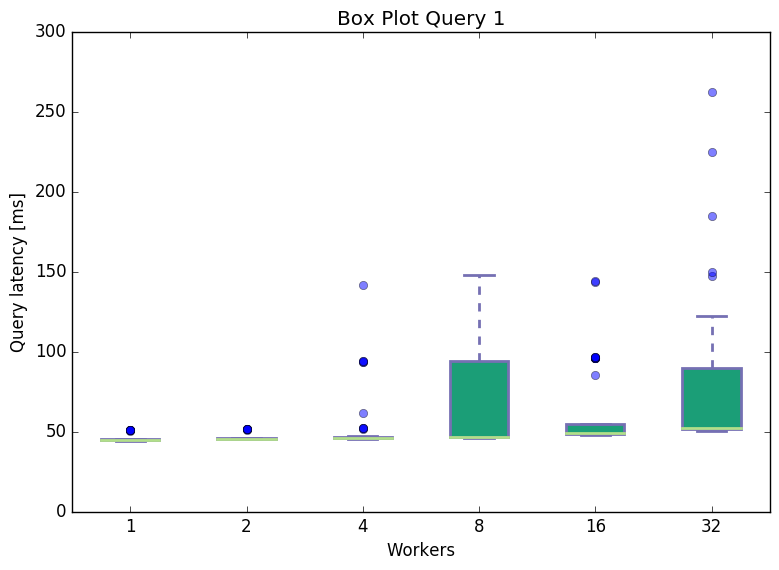
\includegraphics[width=\textwidth]{boxesjs/q1}
    \captionof{figure}{Small Jellyfish}
  \end{minipage}
\end{figure}
\clearpage
\subsection{Query2}
\begin{verbatim}
SELECT n.name WHERE (n) -[e with weight < 4]-> (m)\end{verbatim}

\textbf{Peak Memory: 3'597'452 kb}\\
\textbf{Result size: 36'542}\\
2 Joins and 1 Selection. The joins are not very expensive since we only use about 30\% of the edges.\\\\
\textbf{Dataflow}
\begin{figure}[H]
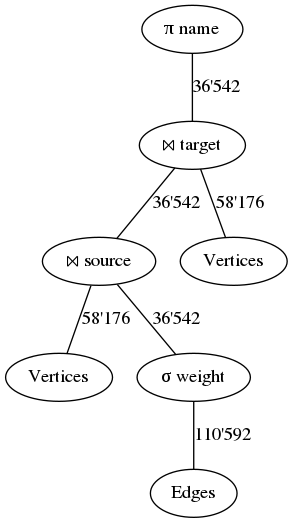
\includegraphics[width=0.4\textwidth]{graph2}
\caption{Dataflow Query2}
\end{figure}
\clearpage
\begin{figure}[!tbp]
  \centering
  \RawFloats
  \begin{minipage}[b]{0.5\textwidth}
    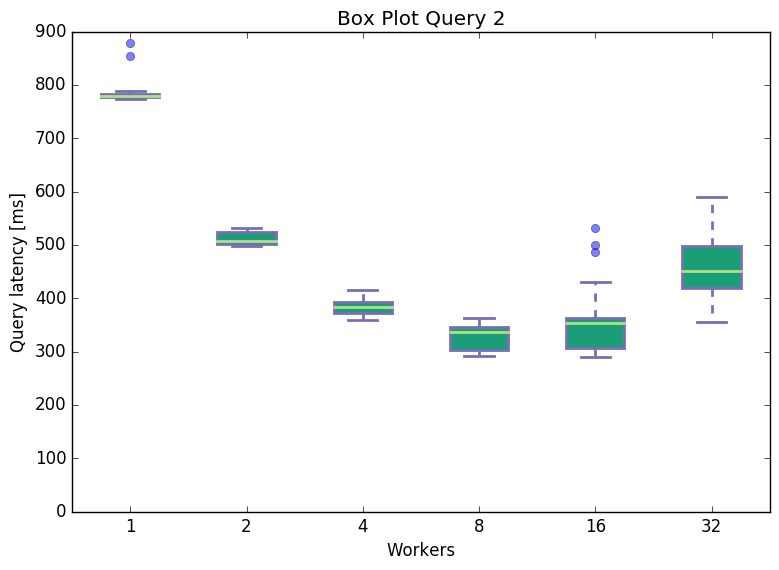
\includegraphics[width=\textwidth]{boxesfl/q2}
    \captionof{figure}{Large Fattree}
  \end{minipage}
  \hfill
  \begin{minipage}[b]{0.5\textwidth}
    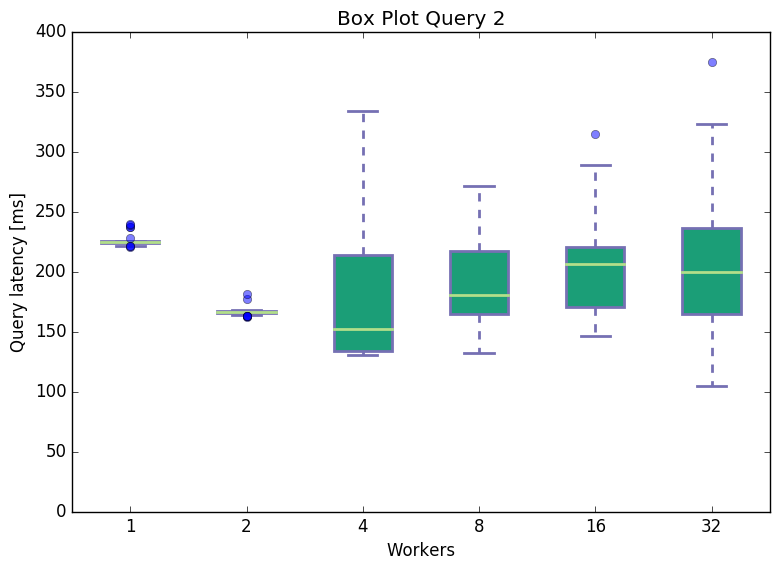
\includegraphics[width=\textwidth]{boxesfs/q2}
    \captionof{figure}{Small Fattree}
  \end{minipage}
\end{figure}
\begin{figure}[!tbp]
  \centering
  \RawFloats
  \begin{minipage}[b]{0.5\textwidth}
    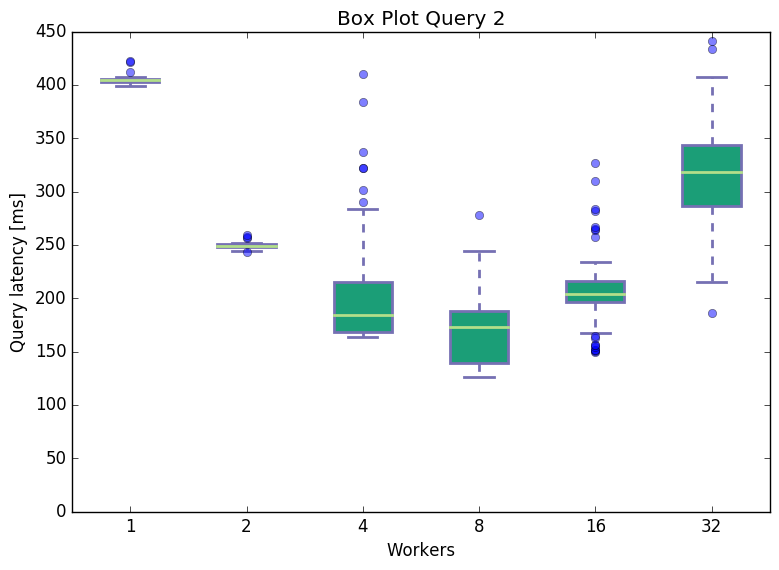
\includegraphics[width=\textwidth]{boxesjl/q2}
    \captionof{figure}{Large Jellyfish}
  \end{minipage}
  \hfill
  \begin{minipage}[b]{0.5\textwidth}
    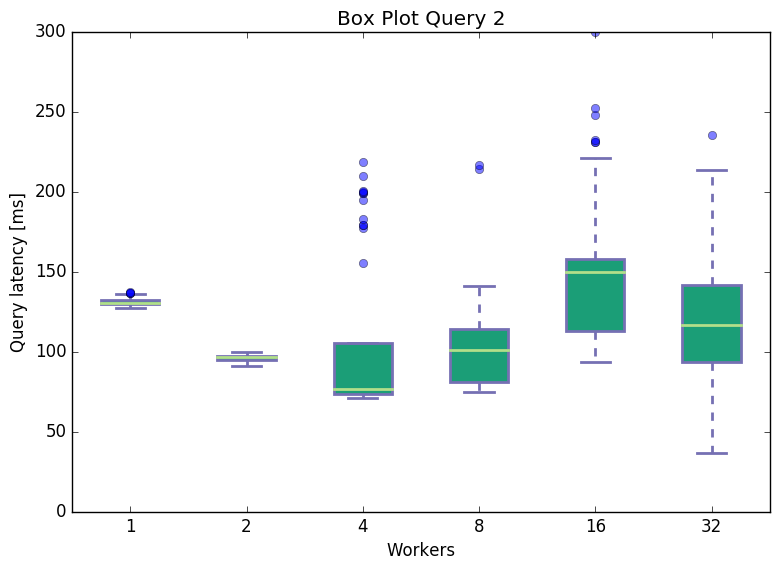
\includegraphics[width=\textwidth]{boxesjs/q2}
    \captionof{figure}{Small Jellyfish}
  \end{minipage}
\end{figure}
\clearpage
\subsection{Query3}
\begin{verbatim}
SELECT n.name WHERE (n:switch) -> (m with position = 'distribution')\end{verbatim}

\textbf{Peak Memory: 1'433'376 kb}\\
\textbf{Result size: 55'296}\\
2 Joins and 2 Selections. I expected this query to be a little bit slower since we are using all the edges in the joins, but it is only a tiny bit slower than Query 2.\\\\
\textbf{Dataflow}
\begin{figure}[H]
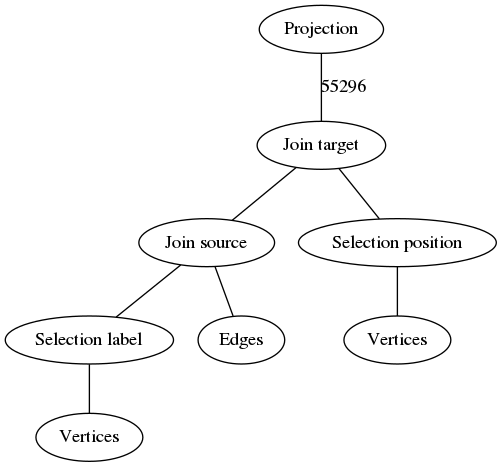
\includegraphics[width=0.6\textwidth]{graph3}
\caption{Dataflow Query3}
\end{figure}
\clearpage
\begin{figure}[!tbp]
  \centering
  \RawFloats
  \begin{minipage}[b]{0.5\textwidth}
    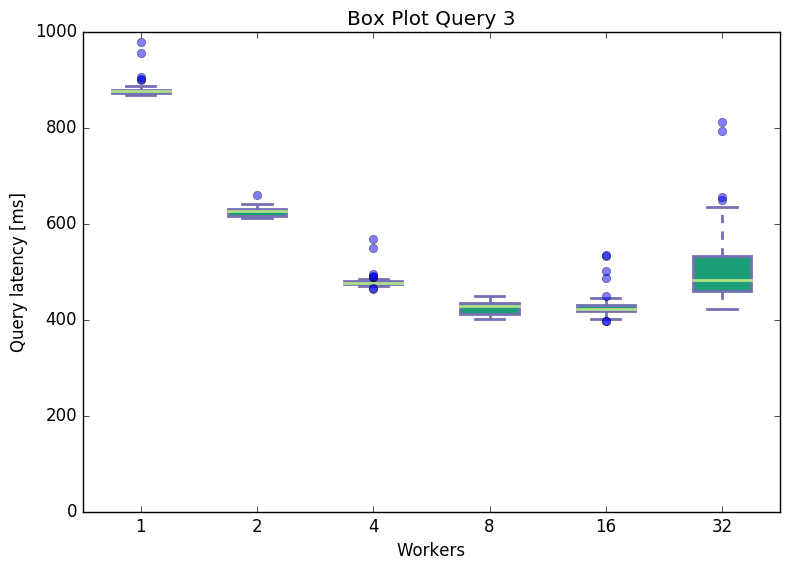
\includegraphics[width=\textwidth]{boxesfl/q3}
    \captionof{figure}{Large Fattree}
  \end{minipage}
  \hfill
  \begin{minipage}[b]{0.5\textwidth}
    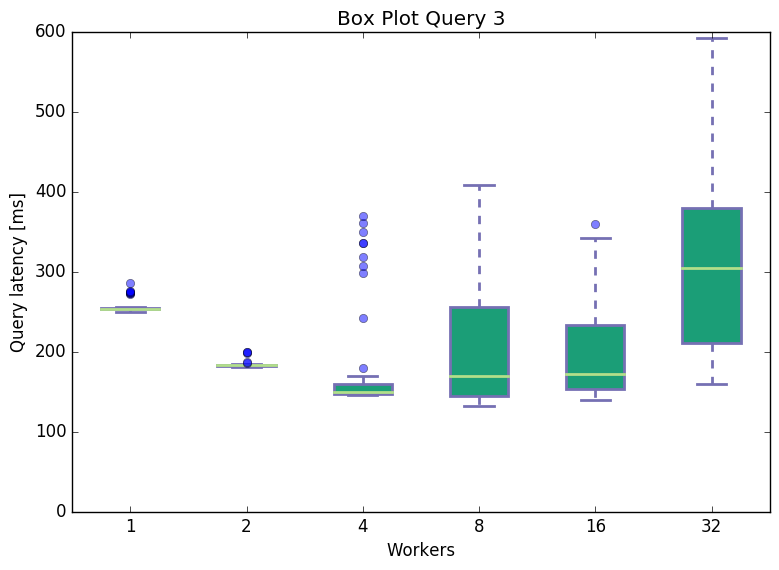
\includegraphics[width=\textwidth]{boxesfs/q3}
    \captionof{figure}{Small Fattree}
  \end{minipage}
\end{figure}
\begin{figure}[!tbp]
  \centering
  \RawFloats
  \begin{minipage}[b]{0.5\textwidth}
    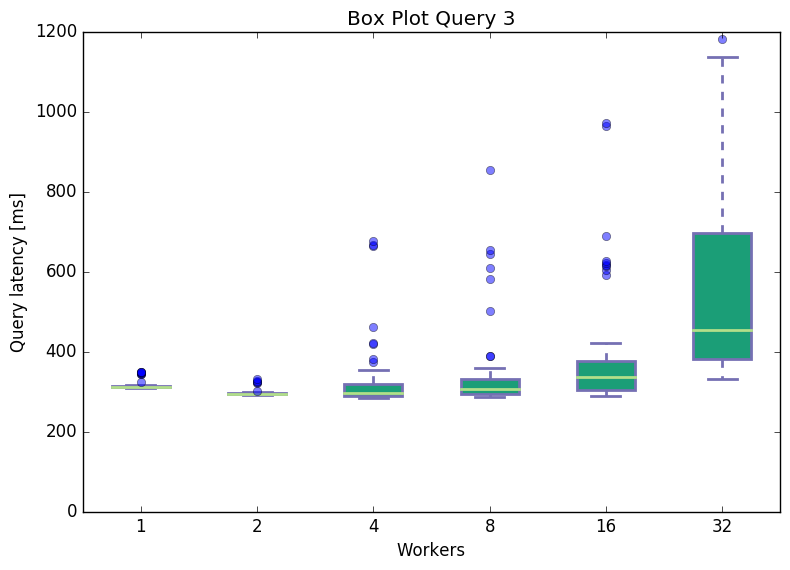
\includegraphics[width=\textwidth]{boxesjl/q3}
    \captionof{figure}{Large Jellyfish}
  \end{minipage}
  \hfill
  \begin{minipage}[b]{0.5\textwidth}
    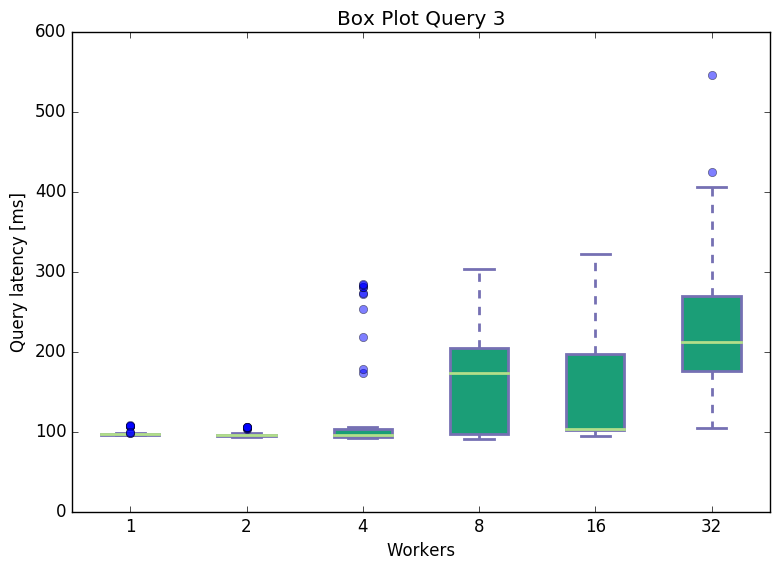
\includegraphics[width=\textwidth]{boxesjs/q3}
    \captionof{figure}{Small Jellyfish}
  \end{minipage}
\end{figure}
\clearpage
\subsection{Query4}
\begin{verbatim}
SELECT n.name WHERE (n with position = 'distribution')
-[e with weight > 8]-> (m with position = 'access')\end{verbatim}

\textbf{Peak Memory: 1'114'896 kb}\\
\textbf{Result size: 3'097}\\
2 Joins and 3 Selections. Even though this query has more constraints than Query 2 and 3, it is faster since we only use 10\% of the edges in the joins. \\\\
\textbf{Dataflow}
\begin{figure}[H]
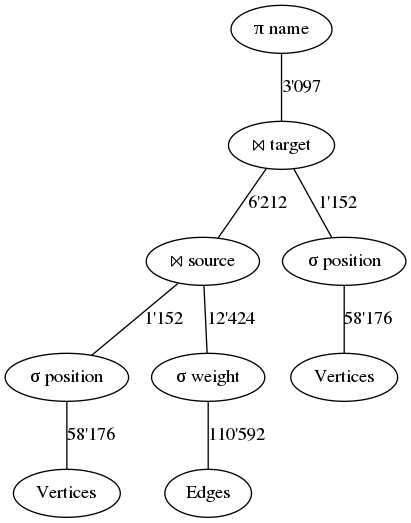
\includegraphics[width=0.6\textwidth]{graph4}
\caption{Dataflow Query4}
\end{figure}
\clearpage
\begin{figure}[!tbp]
  \centering
  \RawFloats
  \begin{minipage}[b]{0.5\textwidth}
    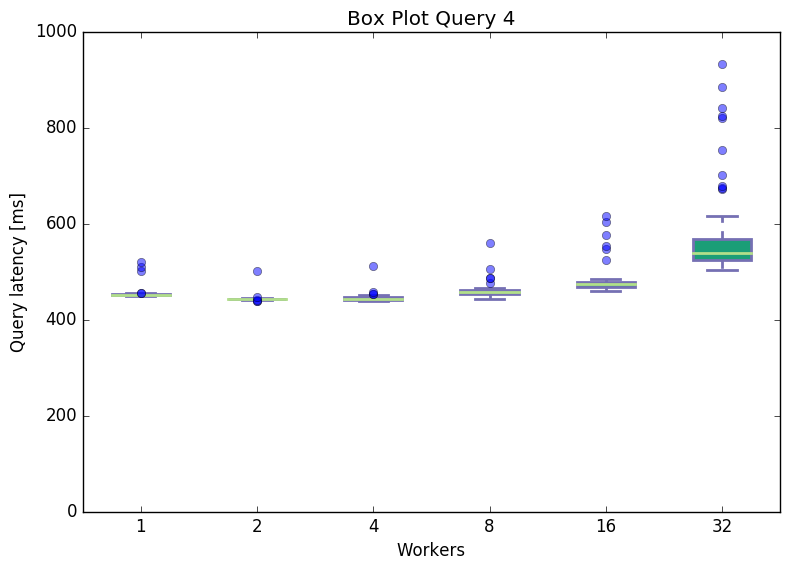
\includegraphics[width=\textwidth]{boxesfl/q4}
    \captionof{figure}{Large Fattree}
  \end{minipage}
  \hfill
  \begin{minipage}[b]{0.5\textwidth}
    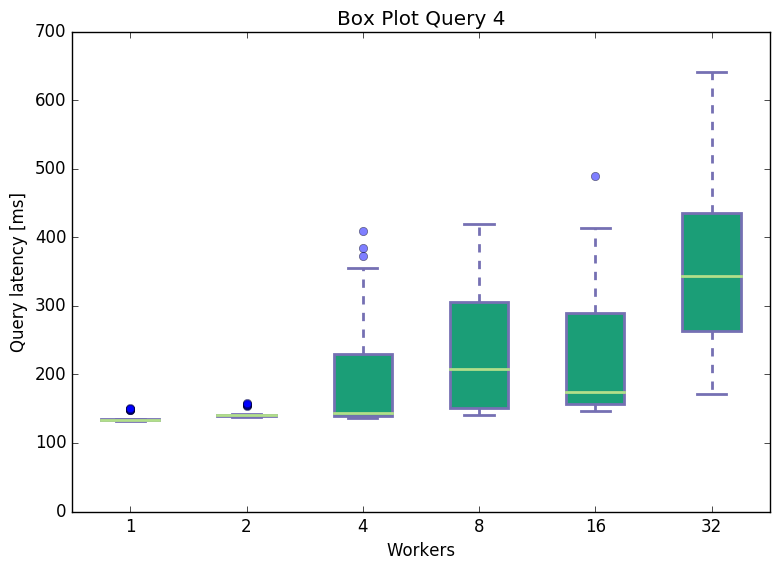
\includegraphics[width=\textwidth]{boxesfs/q4}
    \captionof{figure}{Small Fattree}
  \end{minipage}
\end{figure}
\begin{figure}[!tbp]
  \centering
  \RawFloats
  \begin{minipage}[b]{0.5\textwidth}
    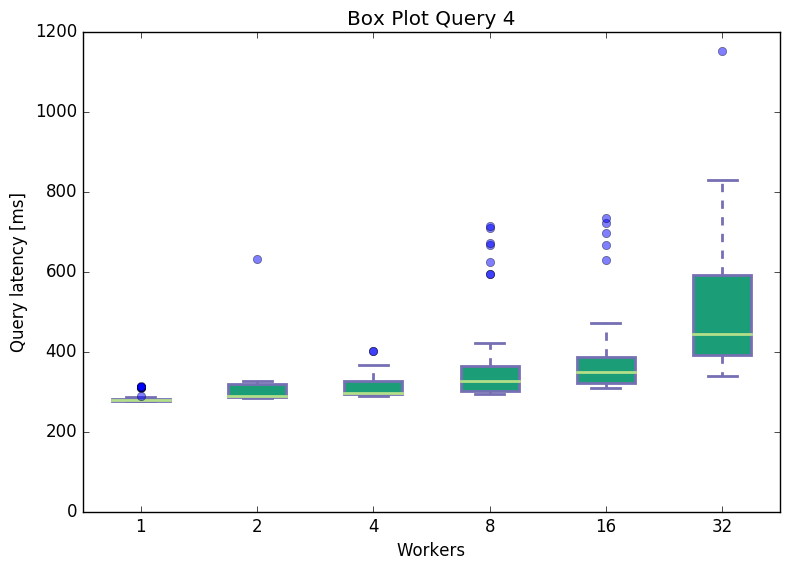
\includegraphics[width=\textwidth]{boxesjl/q4}
    \captionof{figure}{Large Jellyfish}
  \end{minipage}
  \hfill
  \begin{minipage}[b]{0.5\textwidth}
    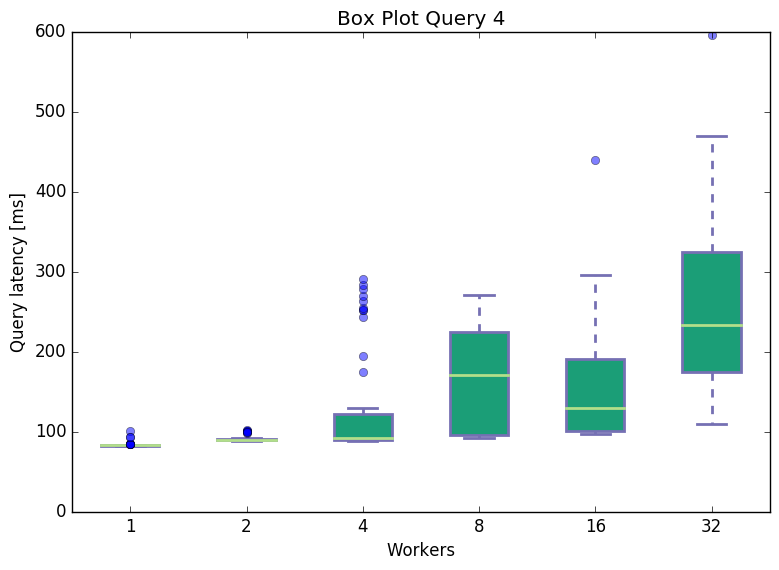
\includegraphics[width=\textwidth]{boxesjs/q4}
    \captionof{figure}{Small Jellyfish}
  \end{minipage}
\end{figure}
\clearpage

\subsection{Query5}
\begin{verbatim}
SELECT v.name WHERE (u WITH position = 'access')
 -> (v WITH position = 'distribution')
 -> (w WITH position = 'core')\end{verbatim}
\textbf{Peak Memory: 3'797'976 kb}\\
\textbf{Result size: 663'552}\\
4 Joins and 3 Selections. The last 3 queries all contain multiple query edges and are much slower. Since there is no selection on the edge, this particular query is quite slow even though it has "only" 4 joins.\\\\
\textbf{Dataflow}
\begin{figure}[H]
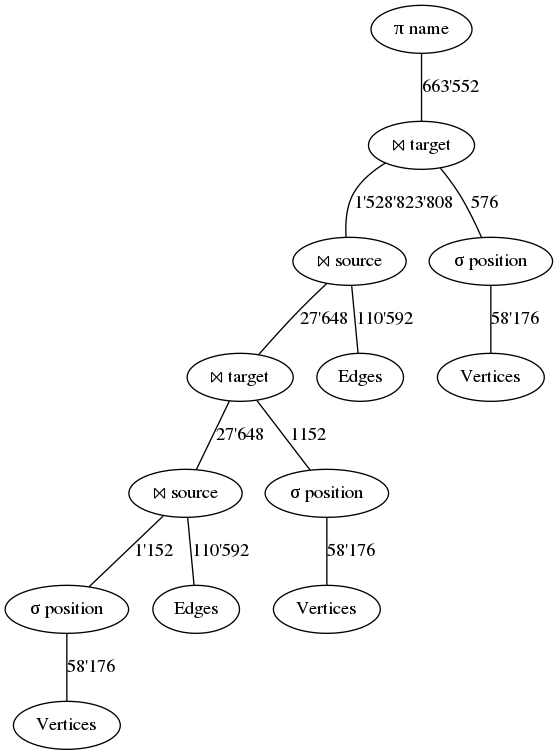
\includegraphics[width=0.6\textwidth]{graph5}
\caption{Dataflow Query5}
\end{figure}
\clearpage
\begin{figure}[!tbp]
  \centering
  \RawFloats
  \begin{minipage}[b]{0.5\textwidth}
    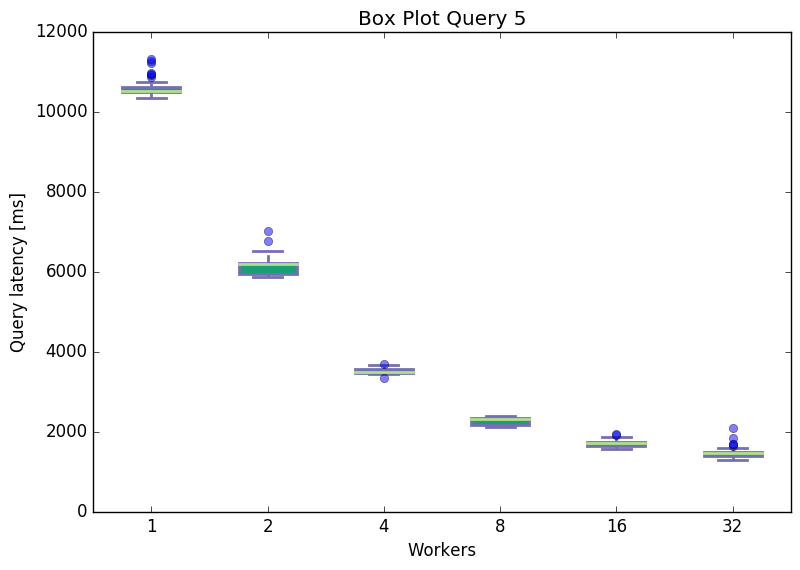
\includegraphics[width=\textwidth]{boxesfl/q5}
    \captionof{figure}{Large Fattree}
  \end{minipage}
  \hfill
  \begin{minipage}[b]{0.5\textwidth}
    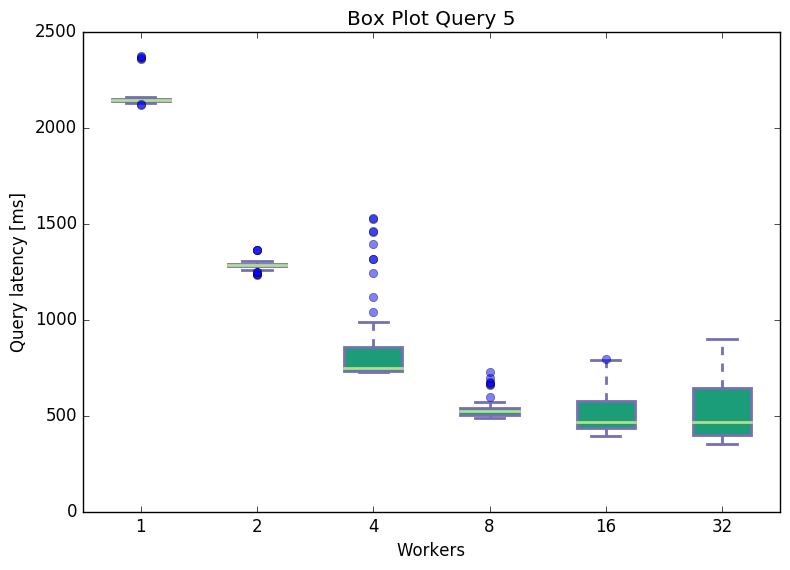
\includegraphics[width=\textwidth]{boxesfs/q5}
    \captionof{figure}{Small Fattree}
  \end{minipage}
\end{figure}
\begin{figure}[!tbp]
  \centering
  \RawFloats
  \begin{minipage}[b]{0.5\textwidth}
    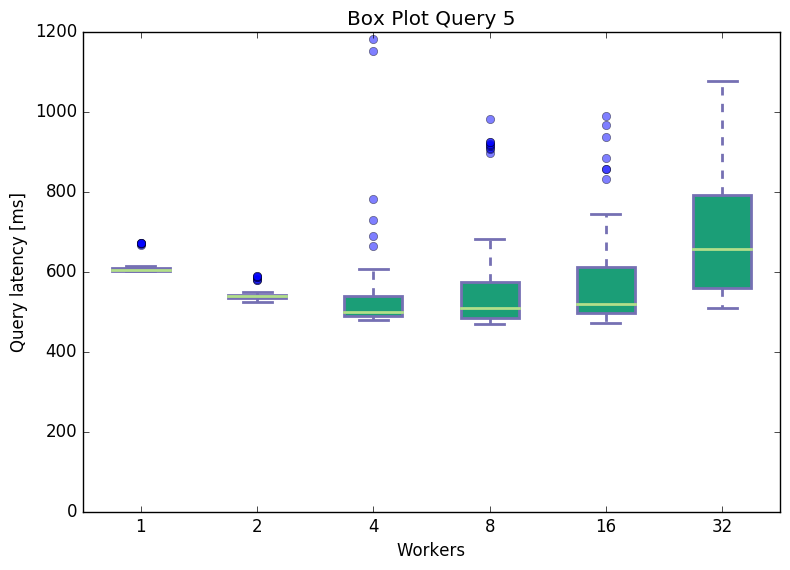
\includegraphics[width=\textwidth]{boxesjl/q5}
    \captionof{figure}{Large Jellyfish}
  \end{minipage}
  \hfill
  \begin{minipage}[b]{0.5\textwidth}
    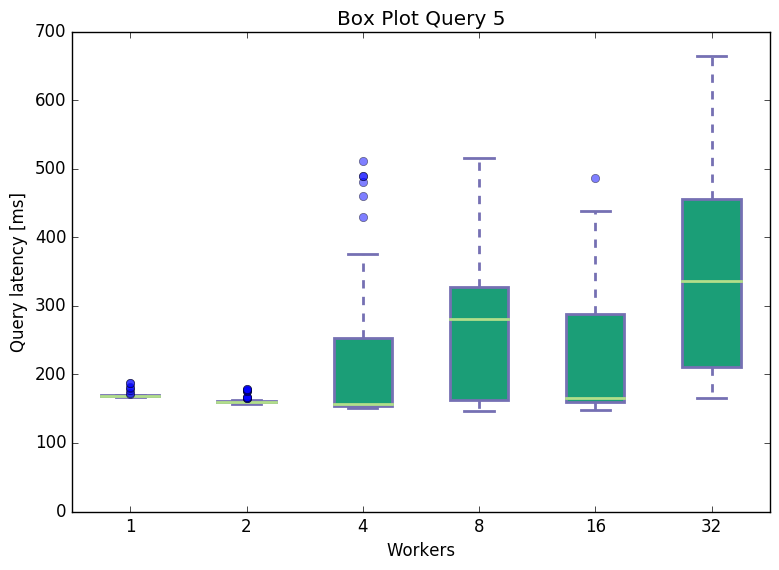
\includegraphics[width=\textwidth]{boxesjs/q5}
    \captionof{figure}{Small Jellyfish}
  \end{minipage}
\end{figure}
\clearpage

\subsection{Query6}
\begin{verbatim}
SELECT v.name WHERE (u WITH position = 'access')
 -[e with weight  < 2]-> (v WITH position = 'distribution')
 -[f with weight > 8]-> (w WITH position = 'core')\end{verbatim}
\textbf{Peak Memory: 1'573'940 kb}\\
\textbf{Result size: 8'334}\\
4 Joins and 5 Selections. Like query 4, the evaluation time goes down as we add more constraints on the edges. Since we have a lot less tuples in the 3rd and 4th join, this query is faster than previous one.\\\\
\textbf{Dataflow}
\begin{figure}[H]
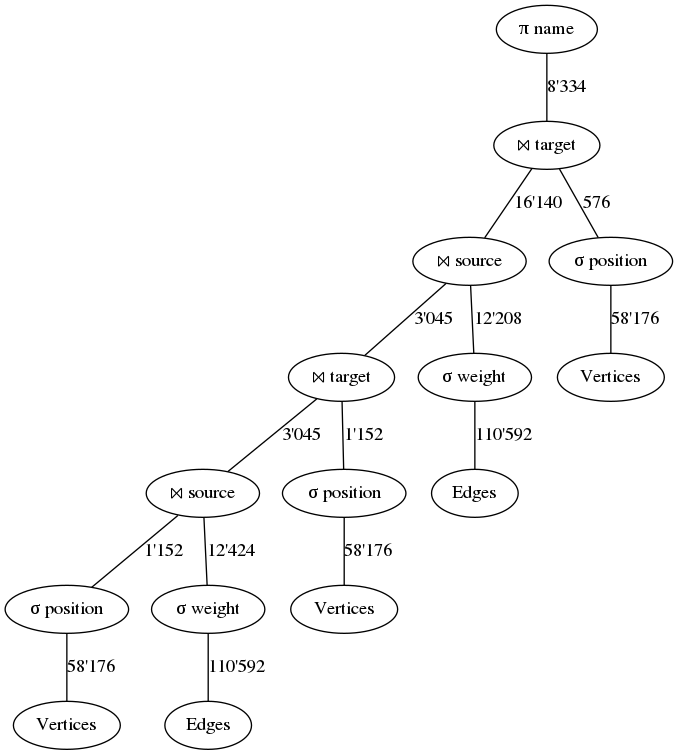
\includegraphics[width=0.8\textwidth]{graph6}
\caption{Dataflow Query6}
\end{figure}
\clearpage
\begin{figure}[!tbp]
  \centering
  \RawFloats
  \begin{minipage}[b]{0.5\textwidth}
    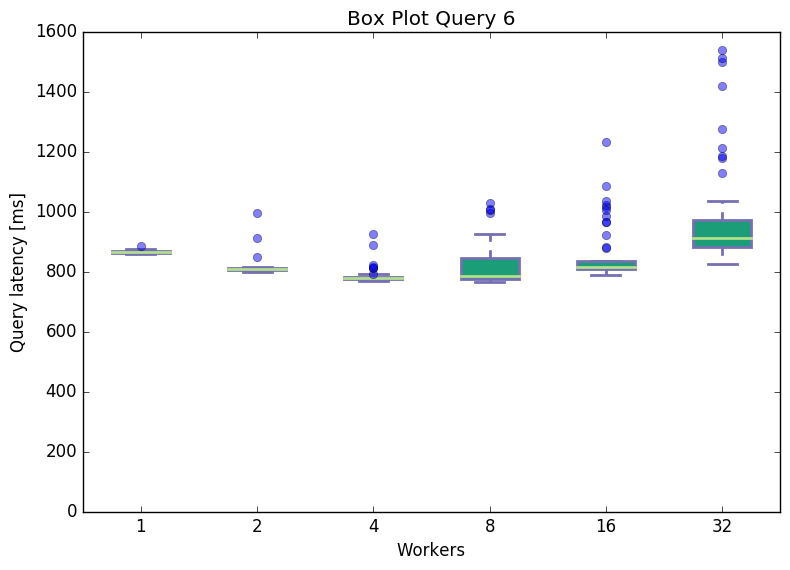
\includegraphics[width=\textwidth]{boxesfl/q6}
    \captionof{figure}{Large Fattree}
  \end{minipage}
  \hfill
  \begin{minipage}[b]{0.5\textwidth}
    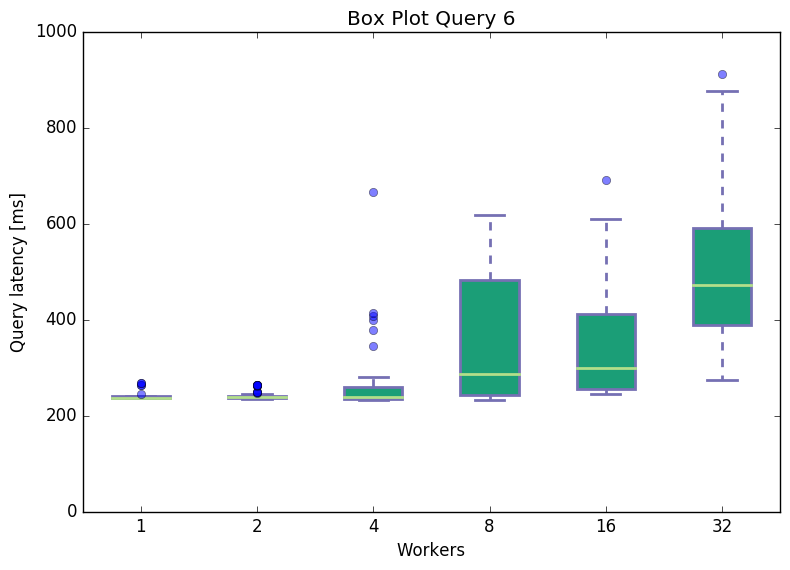
\includegraphics[width=\textwidth]{boxesfs/q6}
    \captionof{figure}{Small Fattree}
  \end{minipage}
\end{figure}
\begin{figure}[!tbp]
  \centering
  \RawFloats
  \begin{minipage}[b]{0.5\textwidth}
    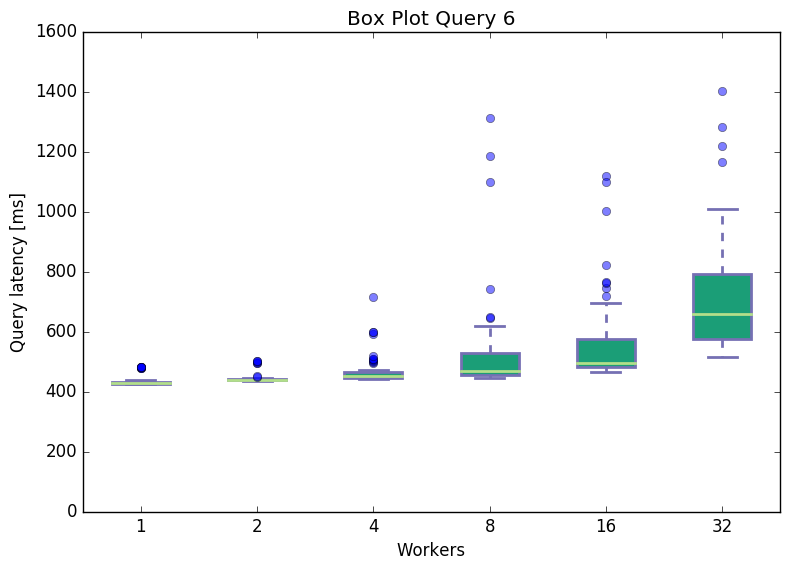
\includegraphics[width=\textwidth]{boxesjl/q6}
    \captionof{figure}{Large Jellyfish}
  \end{minipage}
  \hfill
  \begin{minipage}[b]{0.5\textwidth}
    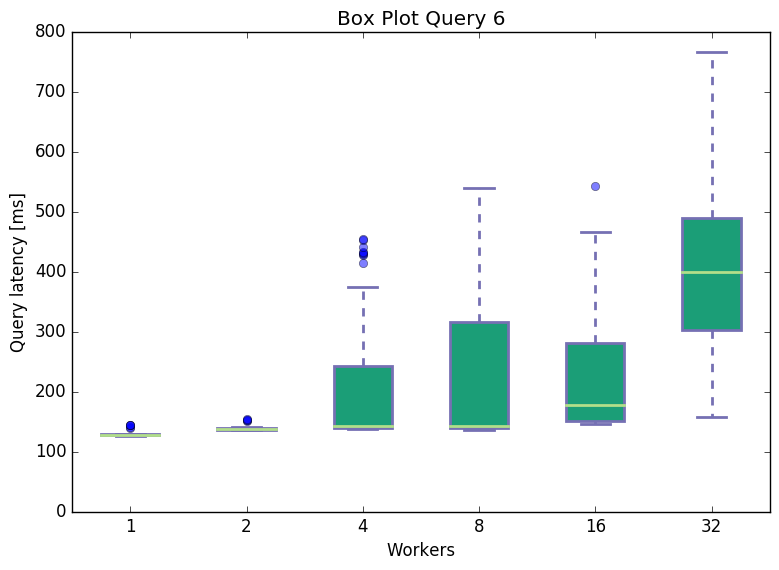
\includegraphics[width=\textwidth]{boxesjs/q6}
    \captionof{figure}{Small Jellyfish}
  \end{minipage}
\end{figure}
\clearpage
\subsection{Query7}
\begin{verbatim}
SELECT v.name WHERE (u WITH position = 'access')
 -[e with weight  < 2]-> (v WITH position = 'distribution')
 -[f with weight  < 2]-> (w WITH position = 'core')
 -[g with weight  < 2]-> (x WITH position = 'distribution')\end{verbatim}
\textbf{Peak Memory: 2'210'824 kb}\\
\textbf{Result size: 49'956}\\
6 Joins and 7 Selections. This is probably the most interesting result. We add two more joins to the query, but we restrict the number of edges used in all the joins dramatically. This consequently leads to a surprisingly low evaluation time, almost on the level as query 5. This demonstrates how big the impact of the joins is for the evaluation time.\\\\
\textbf{Dataflow}
\begin{figure}[H]
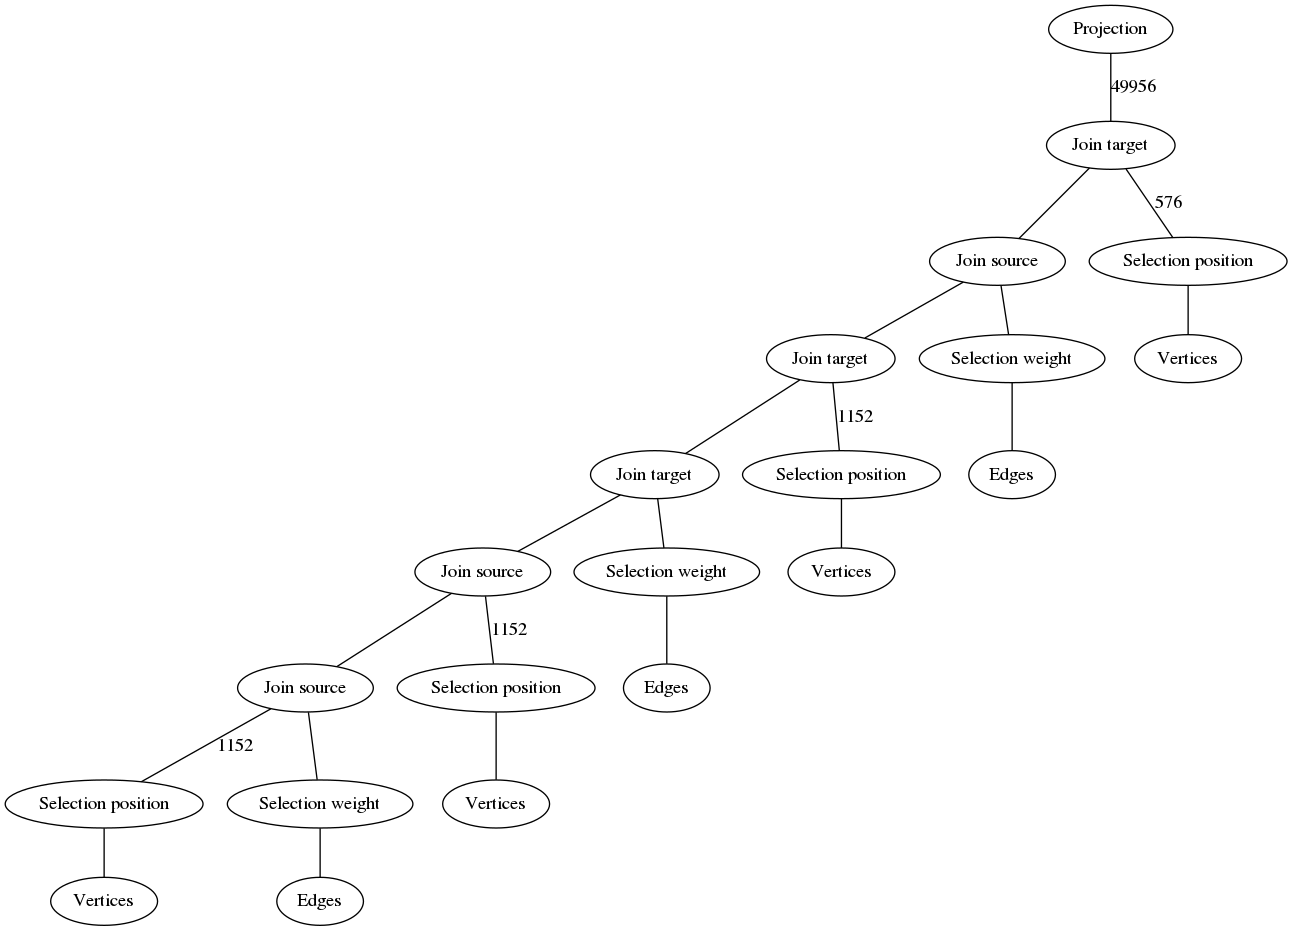
\includegraphics[width=0.8\textwidth]{graph7}
\caption{Dataflow Query7}
\end{figure}
\clearpage
\begin{figure}[!tbp]
  \centering
  \RawFloats
  \begin{minipage}[b]{0.5\textwidth}
    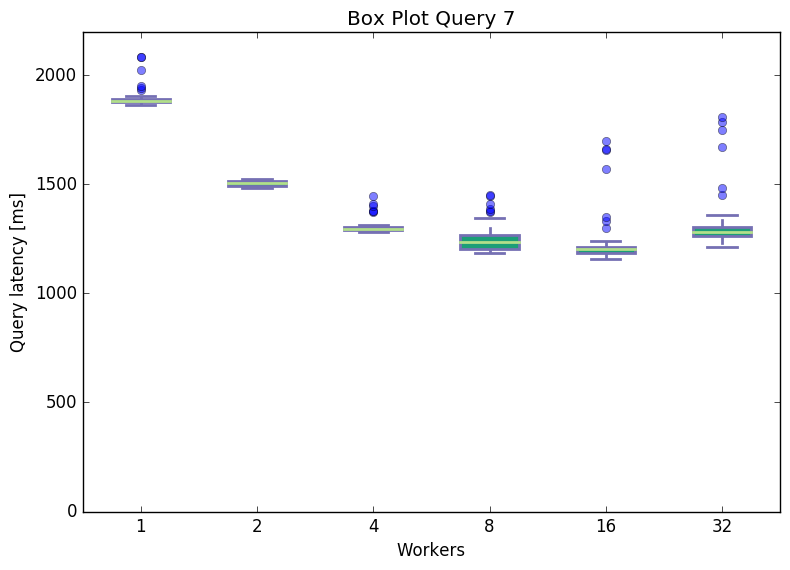
\includegraphics[width=\textwidth]{boxesfl/q7}
    \captionof{figure}{Large Fattree}
  \end{minipage}
  \hfill
  \begin{minipage}[b]{0.5\textwidth}
    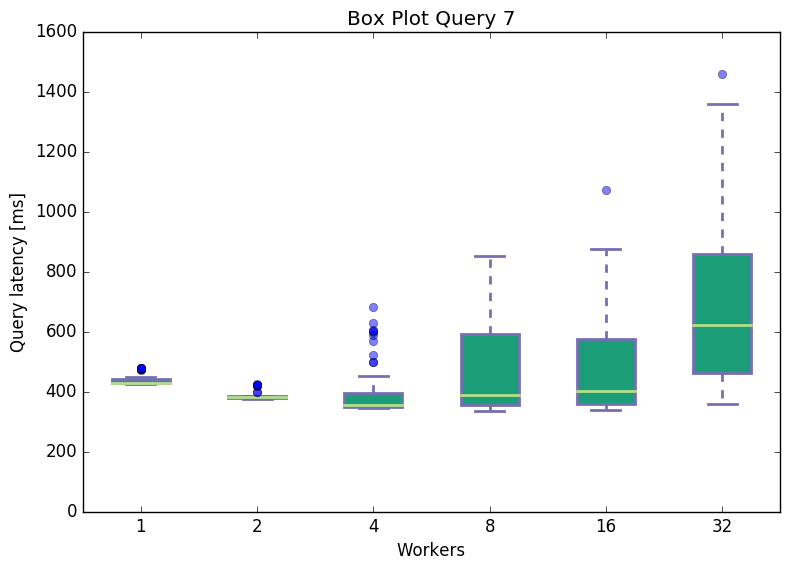
\includegraphics[width=\textwidth]{boxesfs/q7}
    \captionof{figure}{Small Fattree}
  \end{minipage}
\end{figure}
\begin{figure}[!tbp]
  \centering
  \RawFloats
  \begin{minipage}[b]{0.5\textwidth}
    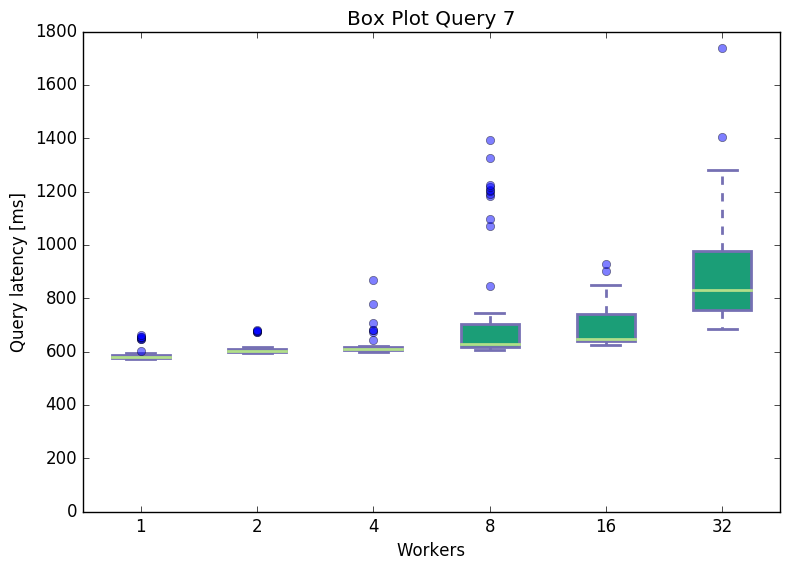
\includegraphics[width=\textwidth]{boxesjl/q7}
    \captionof{figure}{Large Jellyfish}
  \end{minipage}
  \hfill
  \begin{minipage}[b]{0.5\textwidth}
    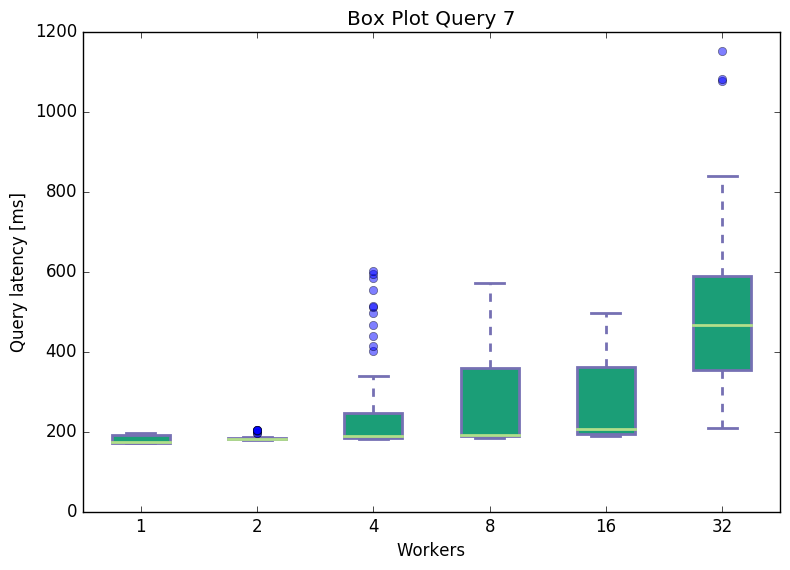
\includegraphics[width=\textwidth]{boxesjs/q7}
    \captionof{figure}{Small Jellyfish}
  \end{minipage}
\end{figure}
\clearpage

\section{Related Work}
In this chapter we give an overview of other existing graph databases and query evluators.

\subsection{SPARQL}
RDF is a directed, labeled graph data format for representing information in the Web. This specification defines the syntax and semantics of the SPARQL query language for RDF. SPARQL can be used to express queries across diverse data sources, whether the data is stored natively as RDF or viewed as RDF via middleware. SPARQL contains capabilities for querying required and optional graph patterns along with their conjunctions and disjunctions. SPARQL also supports extensible value testing and constraining queries by source RDF graph. The results of SPARQL queries can be results sets or RDF graphs.\cite{SPARQL}
\subsection{PQL}
A program query language, PQL for short, is a source language-independent notation to specify program queries and program views. PQL is used as an interface to Static Program Analyzers (SPA), interactive tools that enhance program understanding by answering queries about programs. Queris on global program design as well as searches for detail code patterns are both possible in PQL. Program queries and patterns supported by other notations described in literature and those supported by commercial tools can be written simply and naturally in PQL.\cite {PQL}



\subsection{Green-Marl}
Green-Marl is a domain-specific language (DSL) with high level language construct that allow developers to describe their graph analysis algorithms intuitively, but expose the data-level parallelism inherent in the algorithms. Green-Marl comes with its own compiler which translates high-level algorithmic description written in Green-Marl into an efficient C++ implementation by exploiting this exposed datalevel parallelism. Furthermore, the Green-Marl compiler applies a set of optimizations that take advantage of the high-level semantic knowledge encoded in the Green-Marl DSL. Most graph analysis algorithms can be written very intuitively with Green-Marl and experimental results show that the compiler-generated implementation out of such descriptions performs just as well as or better than highly-tuned handcoded implementations.\cite {Greenmarl}

\subsection{Gremlin}
Developed by the Apache Software Foundation, Gremlin is a query language as well as a graph traversal machine. The graph traversal machine Gremlin consists of three parts that continously interact with each other: first the graph, second the traversal and finally the set of traversers. The traversers move about the graph according to the instructions specified in the traversal, where the result of the computation is the ultimate locations of all halted traversers. A Gremlin machine can be executed over any supporting graph computing system such as an OLTP graph database and/or an OLAP graph processor. The language Gremlin is a functional language implemented in the user’s native programming language. Gremlin supports both imperative and declarative querying.
\cite{Gremlin}


\subsection{SQLGraph}
SQLGraph is a Graph Store that combines existing relational optimizers with a novel schema, in an attempt to give better performance for property graph storage and retrieval than popular noSQL graph stores. The schema combines relational storage for adjacency information with JSON storage for vertex and edge attributes. This particular schema design has benefits compared to a purely relational or purely JSON solution. The query translation mechanism translates Gremlin queries with no side effects into SQL queries so that one can leverage relational query optimizers. \cite{Sun:2015}


\subsection{GraphiQL}
GRAPHiQL is an intuitive query language for graph analytics, which allows developers to reason in terms of nodes and edges rather than the tables and joins which are used in relational databases. GRAPHiQL provides key graph constructs such as looping, recursion, and neighborhood operations. At runtime, GRAPHiQL compiles graph programs into efficient SQL queries that can run on any relational database. \cite {Graphiql}
\clearpage

\section{Summary}

\subsection{Conclusion}

\subsection{Future Work}
\subsection{Acknowledgements}
I would like to thank my supervisors John Liagouris, Desislava Dimitrova and Moritz Hoffmann for their continuous support and help. They provided many meaningful suggestions and proposals. Their expertise and experience was invaluable.\\\\
I would also like to thank Professor Roscoe for taking the time to supervise my thesis.

\clearpage


\bibliography{MA}{}
\bibliographystyle{plain}
\end{document}
